\documentclass[a0,portrait]{a0poster}
\pagestyle{empty}
\setcounter{secnumdepth}{0}
%\usepackage{times}
\usepackage[absolute]{textpos}
\usepackage{graphicx,times}
\usepackage{shapepar}
\usepackage{fancybox}
\usepackage[pdftex,dvipsnames,table]{xcolor}
\usepackage{authdate}
\usepackage[utf8x]{inputenc}
\definecolor{DarkBlue}{rgb}{0.1,0.1,0.5}
\definecolor{Red}{rgb}{0.9,0.0,0.1}
\definecolor{Black}{rgb}{0.0,0.0,0.0}
\definecolor{Green}{rgb}{0.0,0.9,0.1}

\let\Textsize\normalsize
\def\Head#1{\noindent{\vspace{-0.3em}\begin{center}\huge\color{DarkBlue} #1\end{center}}}
\def\LHead#1{\noindent{\LARGE\color{DarkBlue} #1}\smallskip}
\def\Subhead#1{\noindent{\Large\color{RoyalBlue} #1}}
\def\Subsubhead#1{\noindent{\large\color{RoyalBlue}#1}}
\def\Title#1{\noindent{\Huge\color{Red} #1}}
\TPGrid[40mm,40mm]{23}{12}  % 3 - 1 - 7 - 1 - 3 Columns
%\TPGrid[25mm,20mm]{80}{114}  % 1 unit ~ 1 cm
\parindent=0pt
\parskip=0.5\baselineskip
\newcommand{\ddd}{\,\mathrm{d}}

   \setlength{\paperwidth}{87cm}
   \setlength{\paperheight}{119cm}
   \setlength{\textwidth}{87cm}
   \setlength{\textheight}{114cm}

\begin{document}

%%%%%%%%%%%%%%%%%%%%%%%%%%%%%%%%%%%%%%%%%%%%%%%%%%%%%%%%%%%%%%%%%%%%%%%%%%

\begin{textblock}{21}(1,0)
\begin{center}
\shadowbox{
\hspace{2cm}
\begin{minipage}{32cm}
  \Title{\begin{center}A Common GPU n-Dimensional Array for Python and C\end{center}\hspace{1cm}}
\end{minipage}
\hspace{2cm}
}
\end{center}
\end{textblock}

\begin{textblock}{3}(18,0)
\doublebox{
\hspace{1.5cm}
\begin{minipage}{15cm}
\vspace{.5cm}
\LHead{Frédéric Bastien}\\
\LHead{Arnaud Bergeron}\\
\LHead{Andreas Klöckner}\\
\LHead{Pascal Vincent}\\
\LHead{Yoshua Bengio}
\end{minipage}
}
\end{textblock}

%%%%%%%%%%%%%%%%%%%%%%%%%%%%%%%%%%

\begin{textblock}{3}(-.3,0)
\scalebox{0.8}{\includegraphics{UdeM_NoirBleu_logo_Marie_crop.pdf}}
\end{textblock}

\begin{textblock}{20}(-2,1.)
{\color{DarkBlue}{\vrule depth 0pt height 0.5cm width 125cm}}
\end{textblock}

%%%%%%%%%%%%%%%%%%%%%%%%%%%%%%%%%%%

\begin{textblock}{12}(-0.3,1.5)
  \Ovalbox{
    \hspace{1cm}
     \begin{minipage}{35.85cm}
	\Head{Why do we need this?}
           \begin{itemize}
\item Efficient linear algebra is a the core of many scientific applications
\item On the CPU, numpy ndarray provides a standard object (for python at least)
\end{itemize}
\vspace{-1em}
\Head{Why a new implementation?}
\Subsubhead{There are already a number of existing GPU computing codebases:}\\
Theano, PyCUDA/PyOpenCL, CUDAmat, Gnumpy, Thrust, ...
\begin{enumerate}
\item All are incompatible
\item They do not support the full range of numpy ndarray features
\item None support both CUDA and OpenCL
\end{enumerate}
\vspace{0.5cm}
\end{minipage}
\hspace{1cm}
}
 \end{textblock}

%%%%%%%%%%%%%%%%%%%%%%%%%%%%%%%%%%%%%%%%%%%%%%%%

\begin{textblock}{16}(-0.3,3.275)

\Ovalbox{
{\color{Black}
\hspace{1cm}
\begin{minipage}{35.85cm}
\Head{Features desired}

\begin{itemize}
\item Support for varying datatypes
\item Support for an arbitrary number of dimensions
\item Support for strides
\item Support for broadcasting
\item Compatibility with CUDA and OpenCL
\end{itemize}
\Head{Easy to develop}
\begin{itemize}
\item Not always a good idea to make a gpu code work for all memory layout.
  \begin{itemize}
  \item Harder to code
  \item Harder to get efficient
  \end{itemize}
\item Just call \begin{bf}as\_\{contiguous,fortran\}\_memory()\end{bf}
 on inputs!
\end{itemize}
\vspace{0.5cm}
\end{minipage}
\hspace{0.8cm}
}
}
\end{textblock}

%%%%%%%%%%%%%%%%%%%

\begin{textblock}{12}(-0.3,5.5)

\Ovalbox{
{\color{Black}
\hspace{1cm}
\begin{minipage}{35.85cm}
\Head{Strides}
\begin{itemize}
\item Strides is a way to specify how much memory to skip between each element of a dimension.
\begin{itemize}
\item This corresponds to the size of one element times the number of elements
\end{itemize}
\item We can use strides to take submatrix ${\color{cyan!50}B}$ from ${\color{red!50}A}$ without copying any memory.
\begin{itemize}
\item The strides stay the same but the number of elements in each dimension is reduced
\end{itemize}
\end{itemize}
\vspace{-1cm}
\begin{center}
\end{center}
\begin{center}
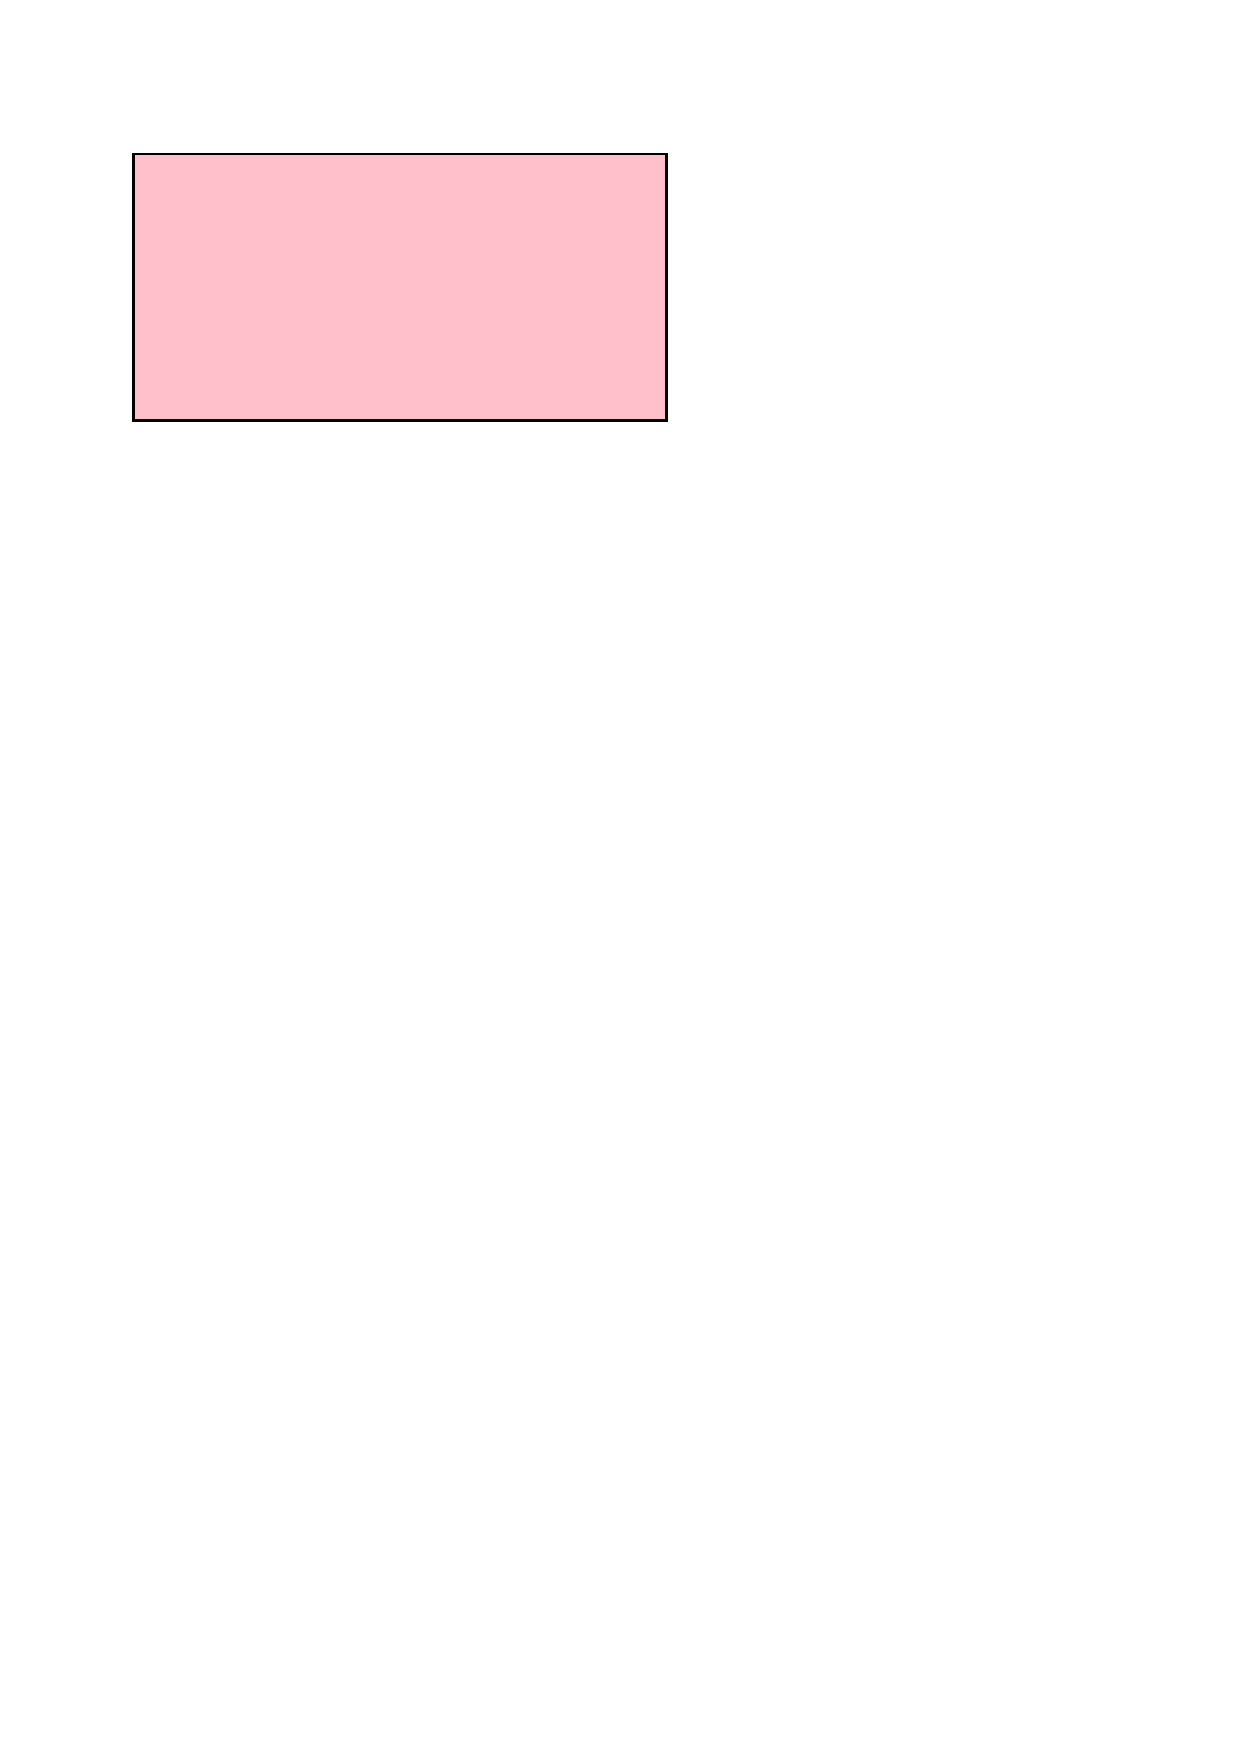
\includegraphics{strides-1}
\hspace{2cm}
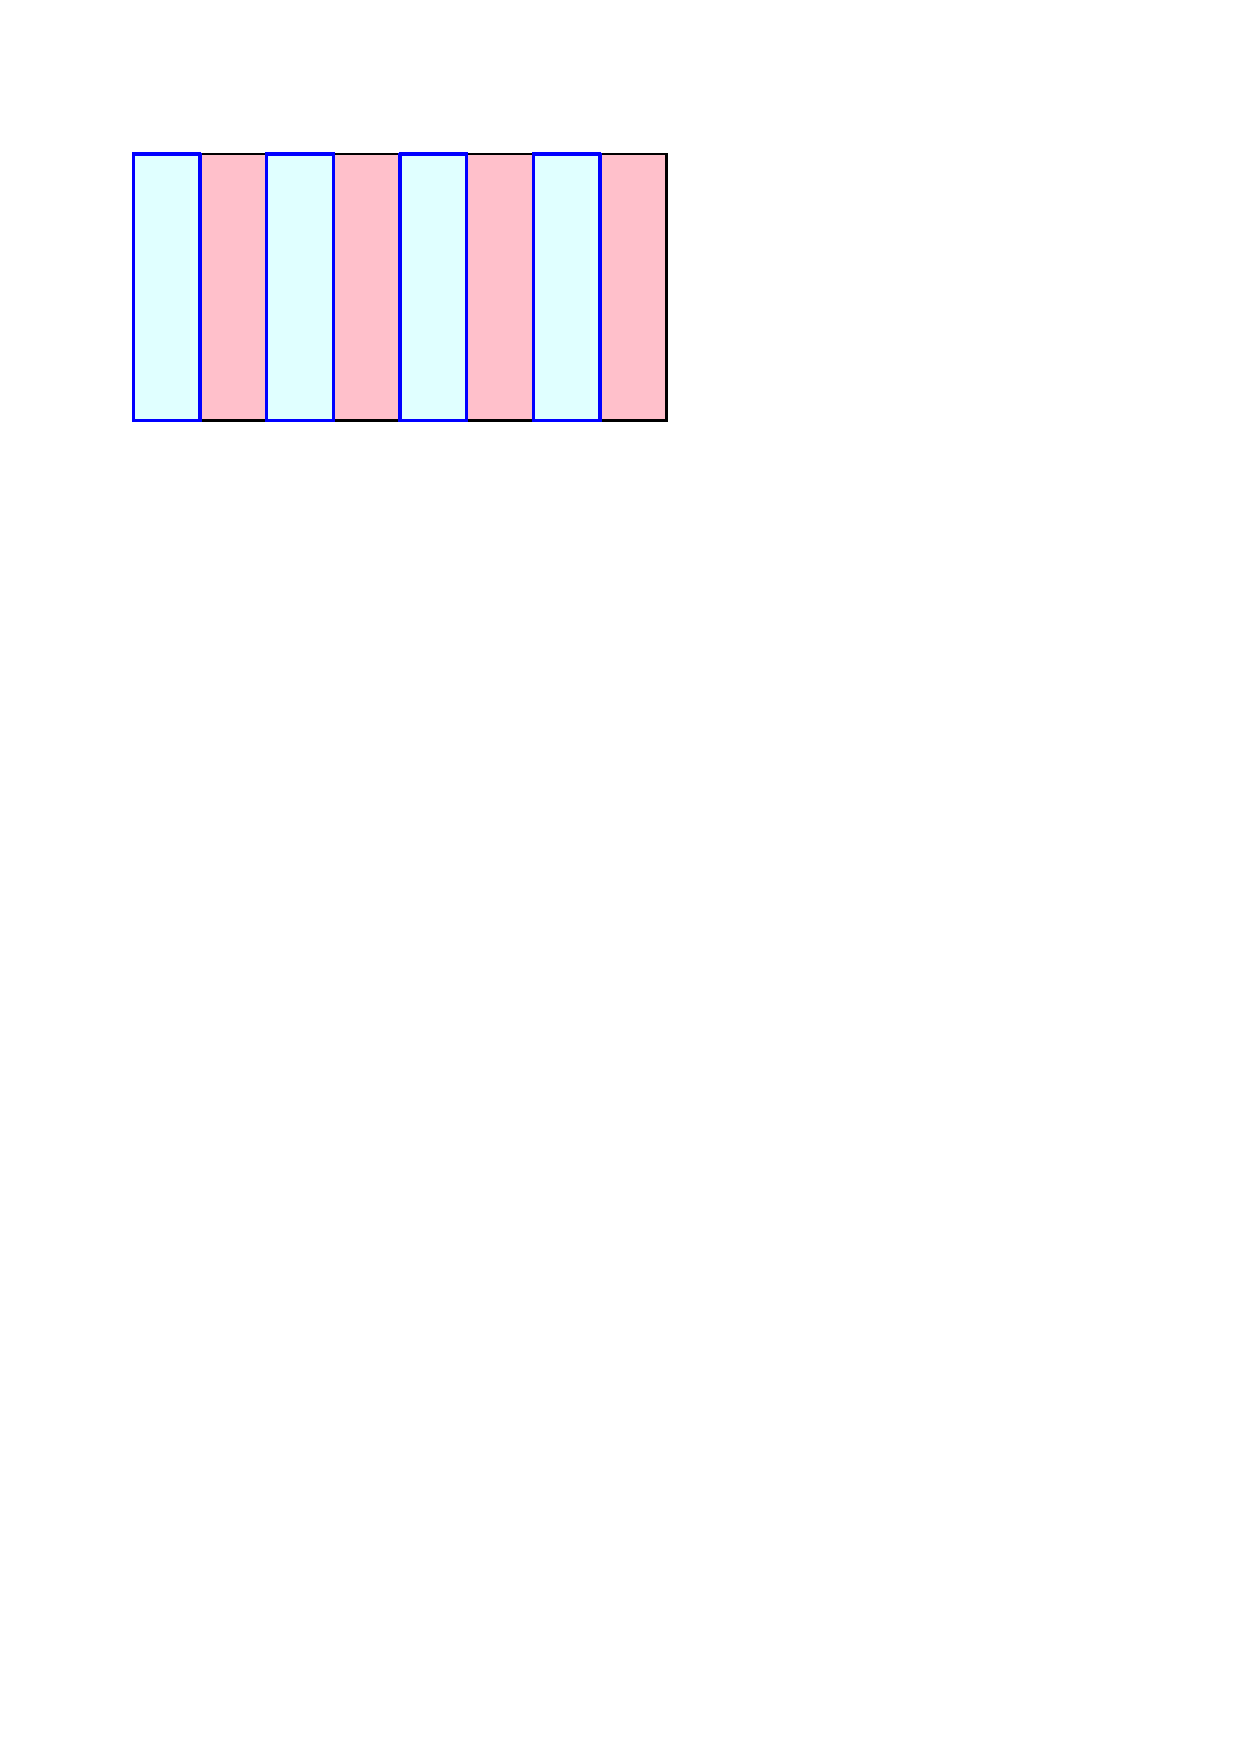
\includegraphics{strides-2}
\end{center}
\vspace{0.2cm}
\end{minipage}
\hspace{1cm}
}}
\end{textblock}
 
%%%%%%%%%%%%%%%%%%%%%%%%%%%%%%%%%%
 
\begin{textblock}{12}(-0.3,7.145)
\Ovalbox{
\hspace{1cm}
\begin{minipage}{35.85cm}
\Head{Broadcasting}
\begin{itemize}
\item We have matrix ${\color{red!50}A}$ (size [8,8]) and we want to add a bias vector ${\color{cyan!50}b}$ (size [8,1]) to it.
\begin{itemize}
\item This doesn't fit the rules for elementwise operations since both objects do not have the same number of elements.
\end{itemize}
\end{itemize}
\begin{center}
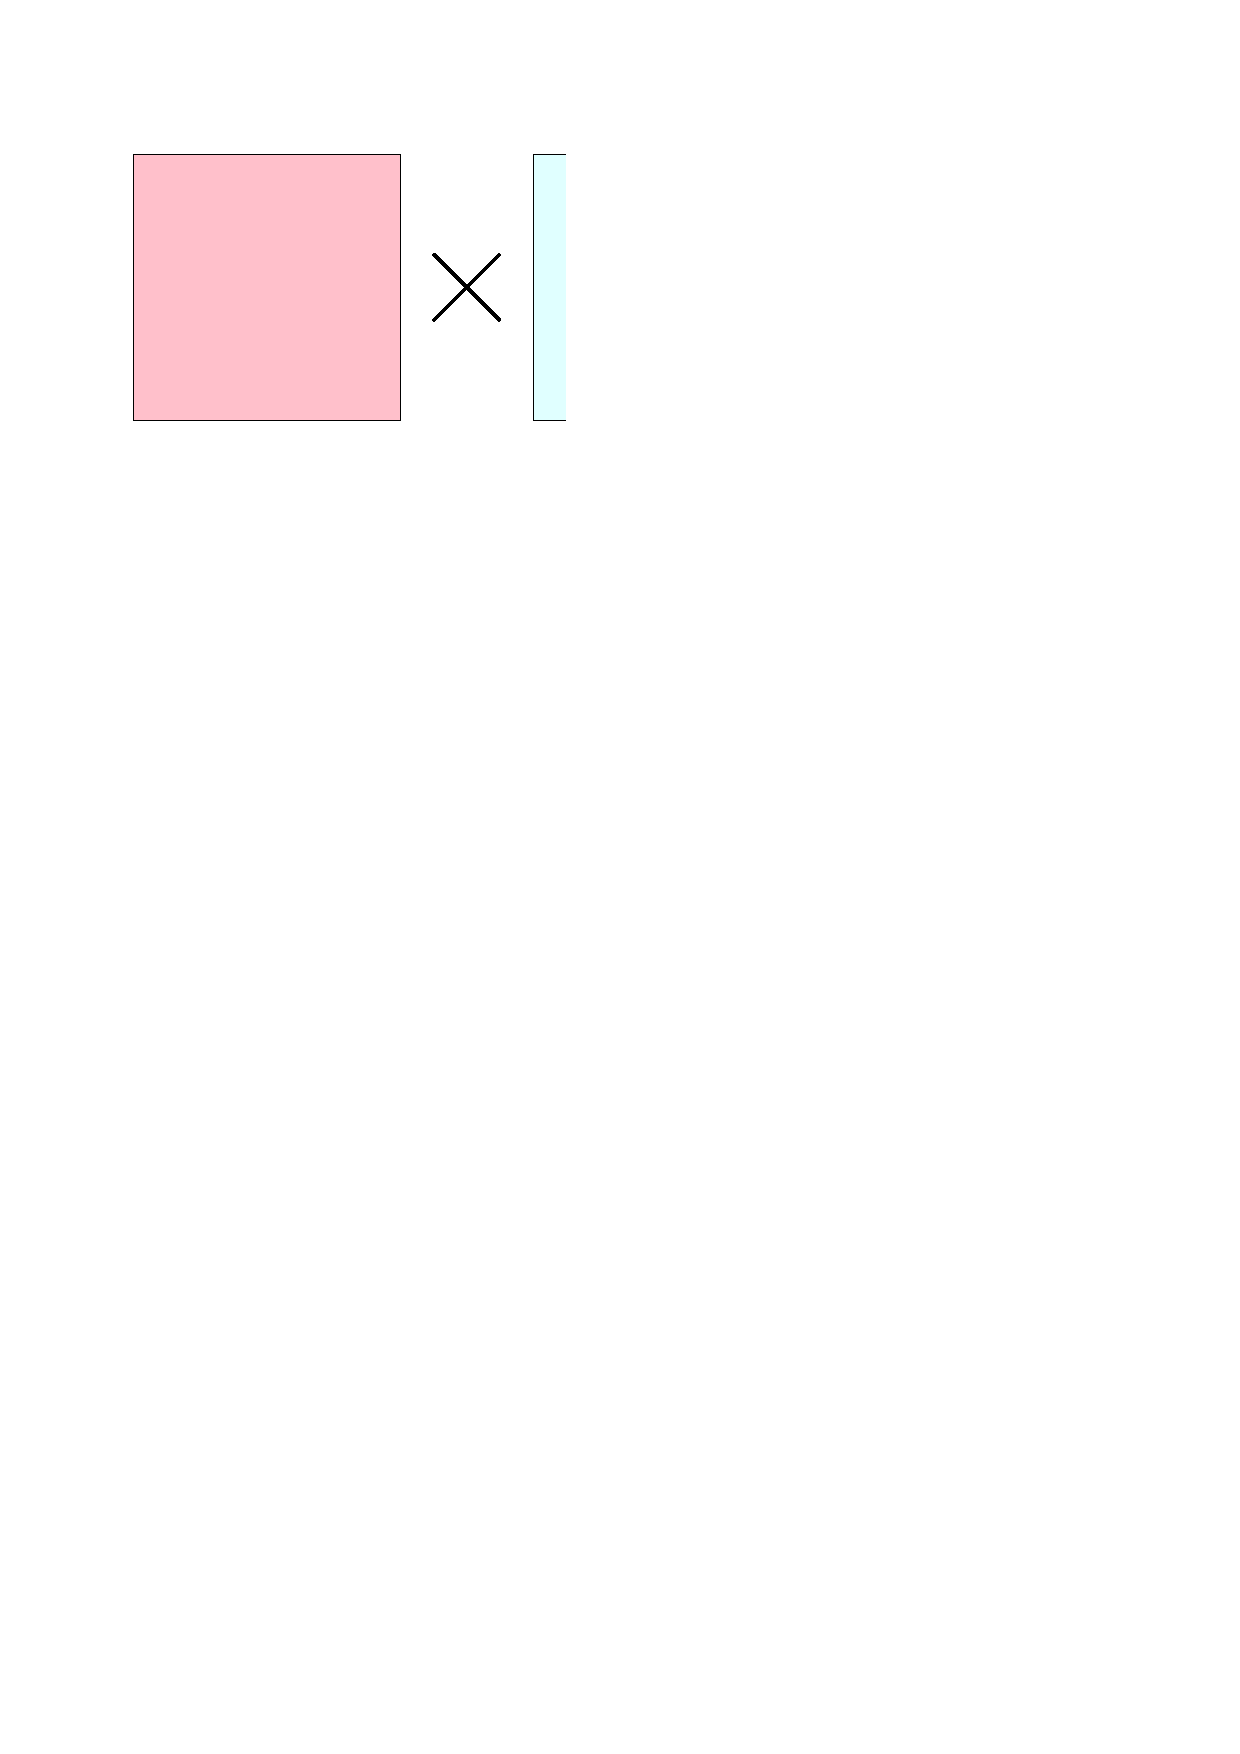
\includegraphics{bcast-1}
\end{center}

\begin{itemize}
\item So we make virtual copies of ${\color{cyan!50}b}$ along the last dimension until it has the same size as ${\color{red!50}A}$.
\begin{itemize}
\item Then we can proceed as usual for elementwise.
\end{itemize}
\end{itemize}
\begin{center}
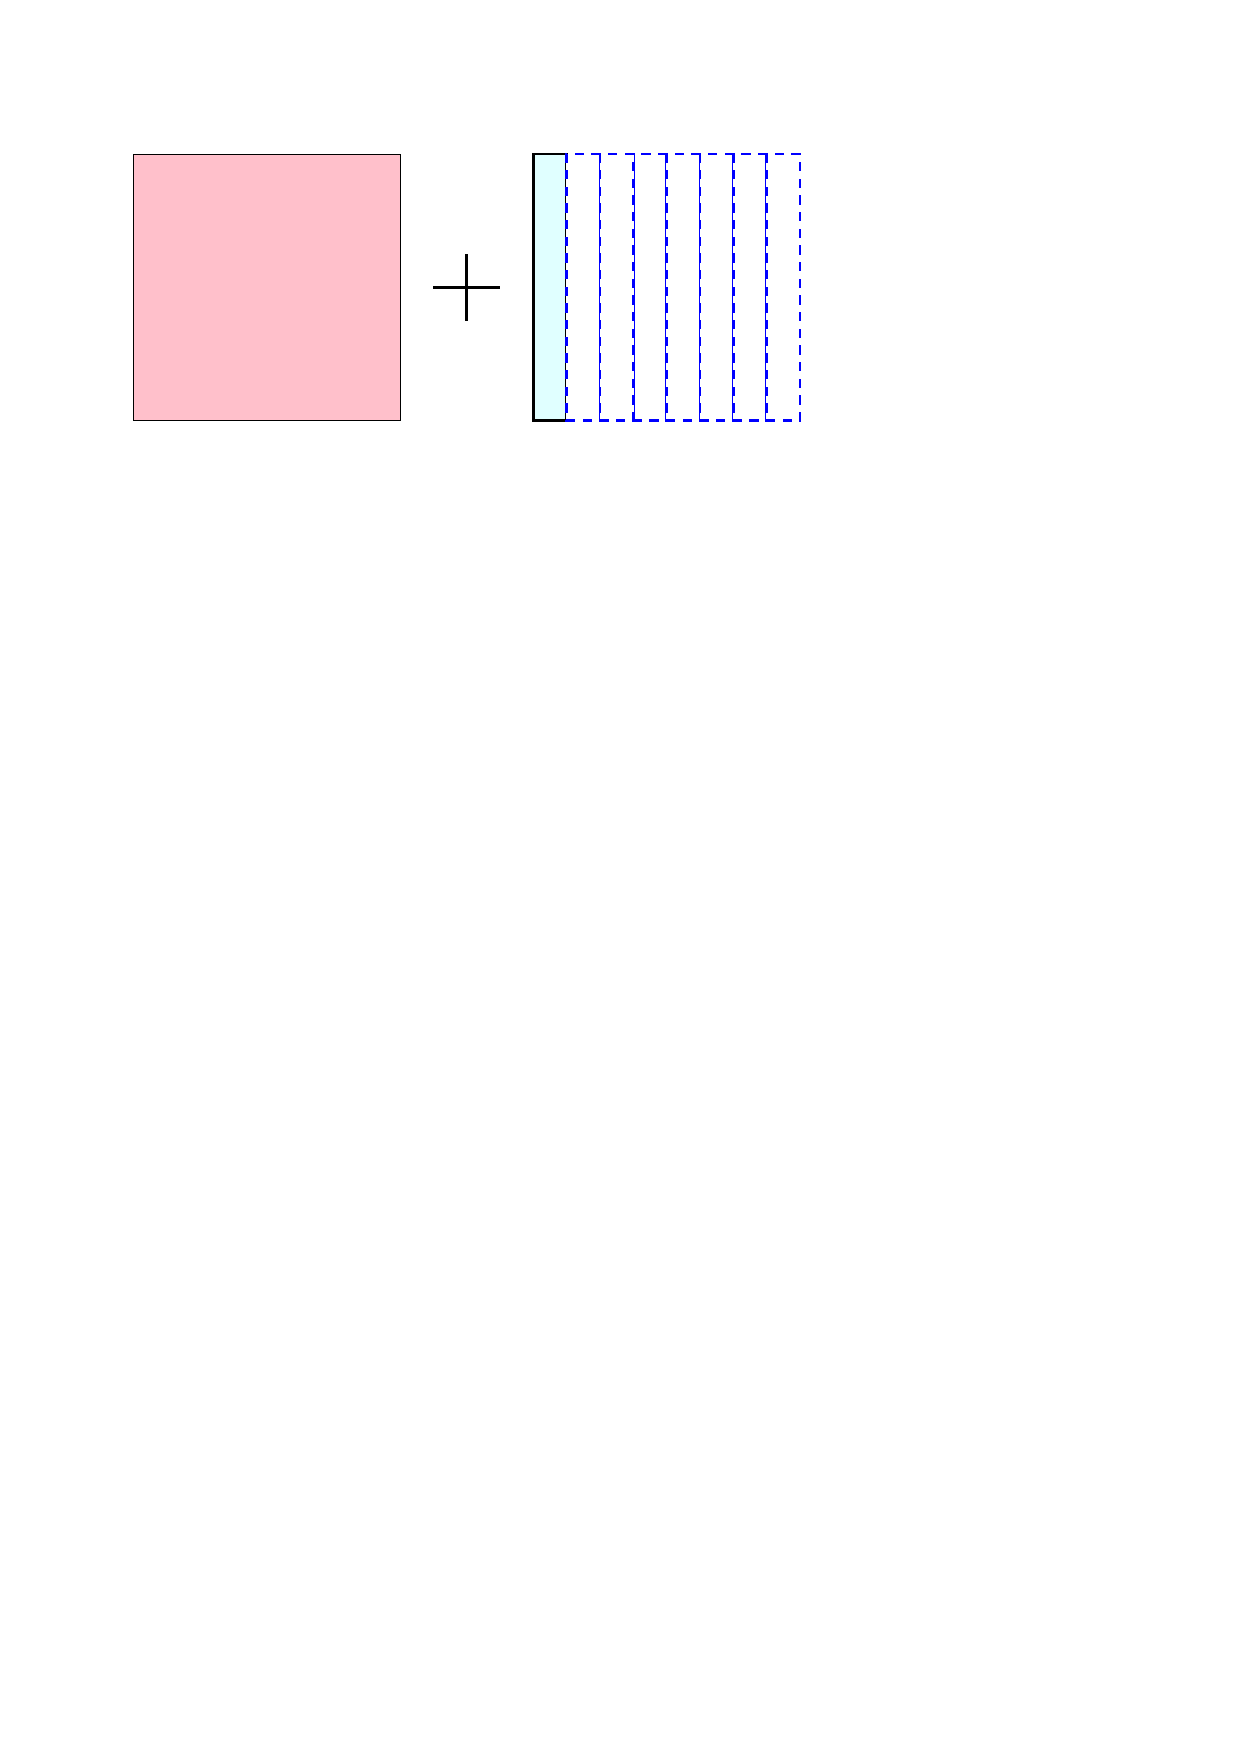
\includegraphics{bcast-2}
\end{center}
\vspace{0.2cm}
\end{minipage}
\hspace{1cm}
}
\end{textblock}

%%%%%%%%%%%%%%%%%%
 
\begin{textblock}{12}(-0.3,9.375)
\Ovalbox{
{\color{Black}
\hspace{1cm}
\begin{minipage}{35.85cm}
\Head{Why has this not been done before?}
\begin{itemize}
\item Hard and time consuming to get right and efficient
\item Certain algorithms cannot work on a general memory layout
\item Indexing computations take up a significant portion of time on the GPU
\end{itemize}
\vspace{0.5cm}
\end{minipage}
\hspace{1cm}
}}
\end{textblock}

%%%%%%%%%%%%%%%%%%%%%%%%%%%%%%%%%%%%%%%%%%%%

 \begin{textblock}{12}(-0.3,10.3)
\Ovalbox{
\hspace{1cm}
\begin{minipage}{35.85cm}
\Head{Comparison of existing implementations}
\large
\rowcolors{2}{RoyalBlue!5}{RoyalBlue!23}
\begin{center}
\begin{tabular}{|l|c|c|c|c|c|}
\hline
Package & strides & broadcast & dimensions & types & backends \\
\hline
\hline
Theano & yes\footnote{\normalsize as number of elements} & yes & any & float32 & CUDA \\
PyCUDA& no & no & any & all & CUDA \\
PyOpenCL & no & no & any & all & OpenCL \\
CUDAMat & no & yes\footnote{\normalsize via a function} & 2 & float32 & CUDA \\
Gnumpy & no & yes & any & float32\footnote{\normalsize and a hackish form of boolean} & CUDA \\
Thrust & no & no & 1 & all & CUDA \\
\hline
\hiderowcolors
Desired & yes & yes & any & all & both \\
\hline
\end{tabular}
\end{center}
\vspace{0.5cm}
\end{minipage}
\hspace{1cm}
}
\end{textblock}

%%%%%%%%%%%%%%%%%%%%%%%%%%%%%%%%%%

\begin{textblock}{12}(11.8,1.5)
\Ovalbox{
\hspace{1cm}
\begin{minipage}{35.85cm}
\Head{Functionality}
\begin{tabular}{ll}
\begin{minipage}{17.5cm}
\Subhead{What we have}
\begin{itemize}
\item data types
\item dimensions
\item strides, views
\item broadcasting
\item elementwise kernels
\item partial reductions
\item support for CUDA and OpenCL
\end{itemize} 
\end{minipage}
&
\begin{minipage}{15cm}
\Subhead{Interfaces}
\begin{itemize}
\item Python
\item C++ interface similar to Numpy C-API (depends on python)
\end{itemize}
\vspace{0.5em}
\Subhead{Missing}
\begin{itemize}
\item assignation
\item reshaping
\item a clean C interface
\end{itemize}
\end{minipage}
\end{tabular}
  \vspace{1cm}
\end{minipage}
\hspace{1cm}
}
\end{textblock}


%%%%%%%%%%%%%%%%%%%%%%%%%%%%%%%%%%%

\begin{textblock}{12}(11.8,3.15)
\Ovalbox{
\hspace{1cm}
\begin{minipage}{35.85cm}
\Head{Element-wise dimension collapsing}
\begin{itemize}
\item Indexing computations are expensive
\item The cost is paid per dimension (irrespective of their size)
\item Suppose we have some elementwise work to do on a 3d tensor ${\color{cyan!50}B}$ that is a view of ${\color{red!50}A}$, but strided in the innnermost dimension.
\begin{itemize}
\item We can merge the two outer dimensions to obtain an equivalent array that accesses the same memory but with easier indexing.
\end{itemize}
\end{itemize}
\begin{center}
\begin{tabular}{m{14cm}m{1cm}m{19cm}}
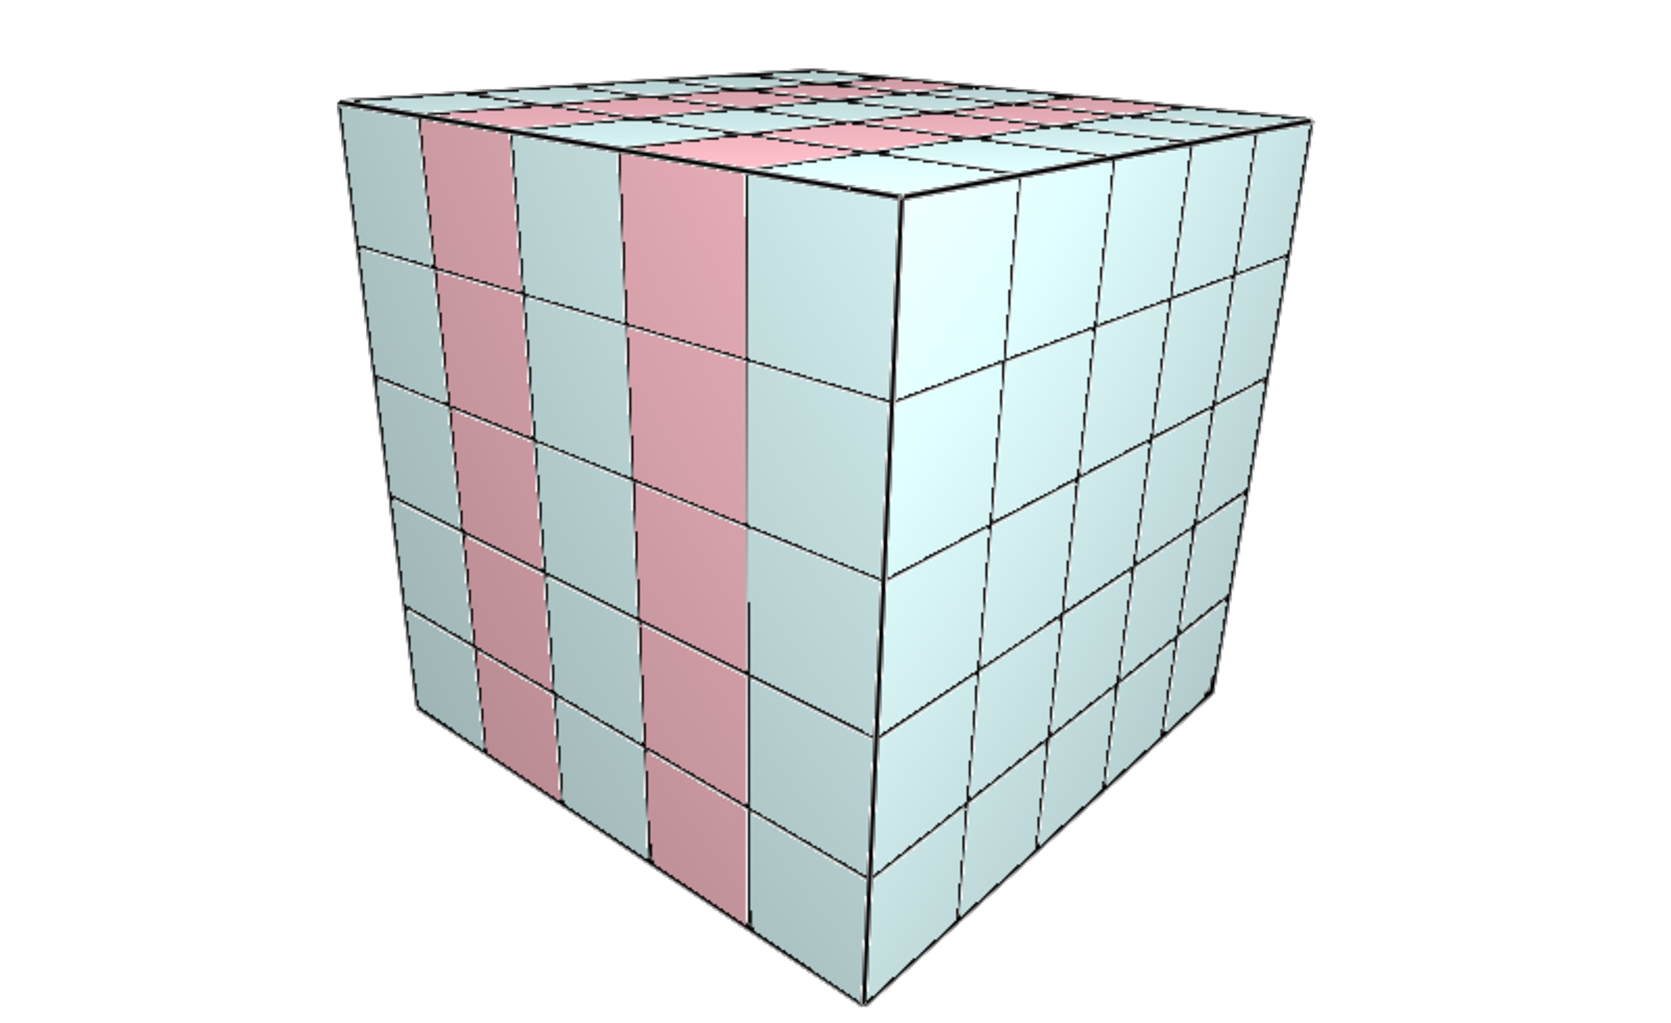
\includegraphics[width=16cm]{dimcoll-1}
&
\vspace{-0.5cm}\hspace{-0.8cm}$\to$
&
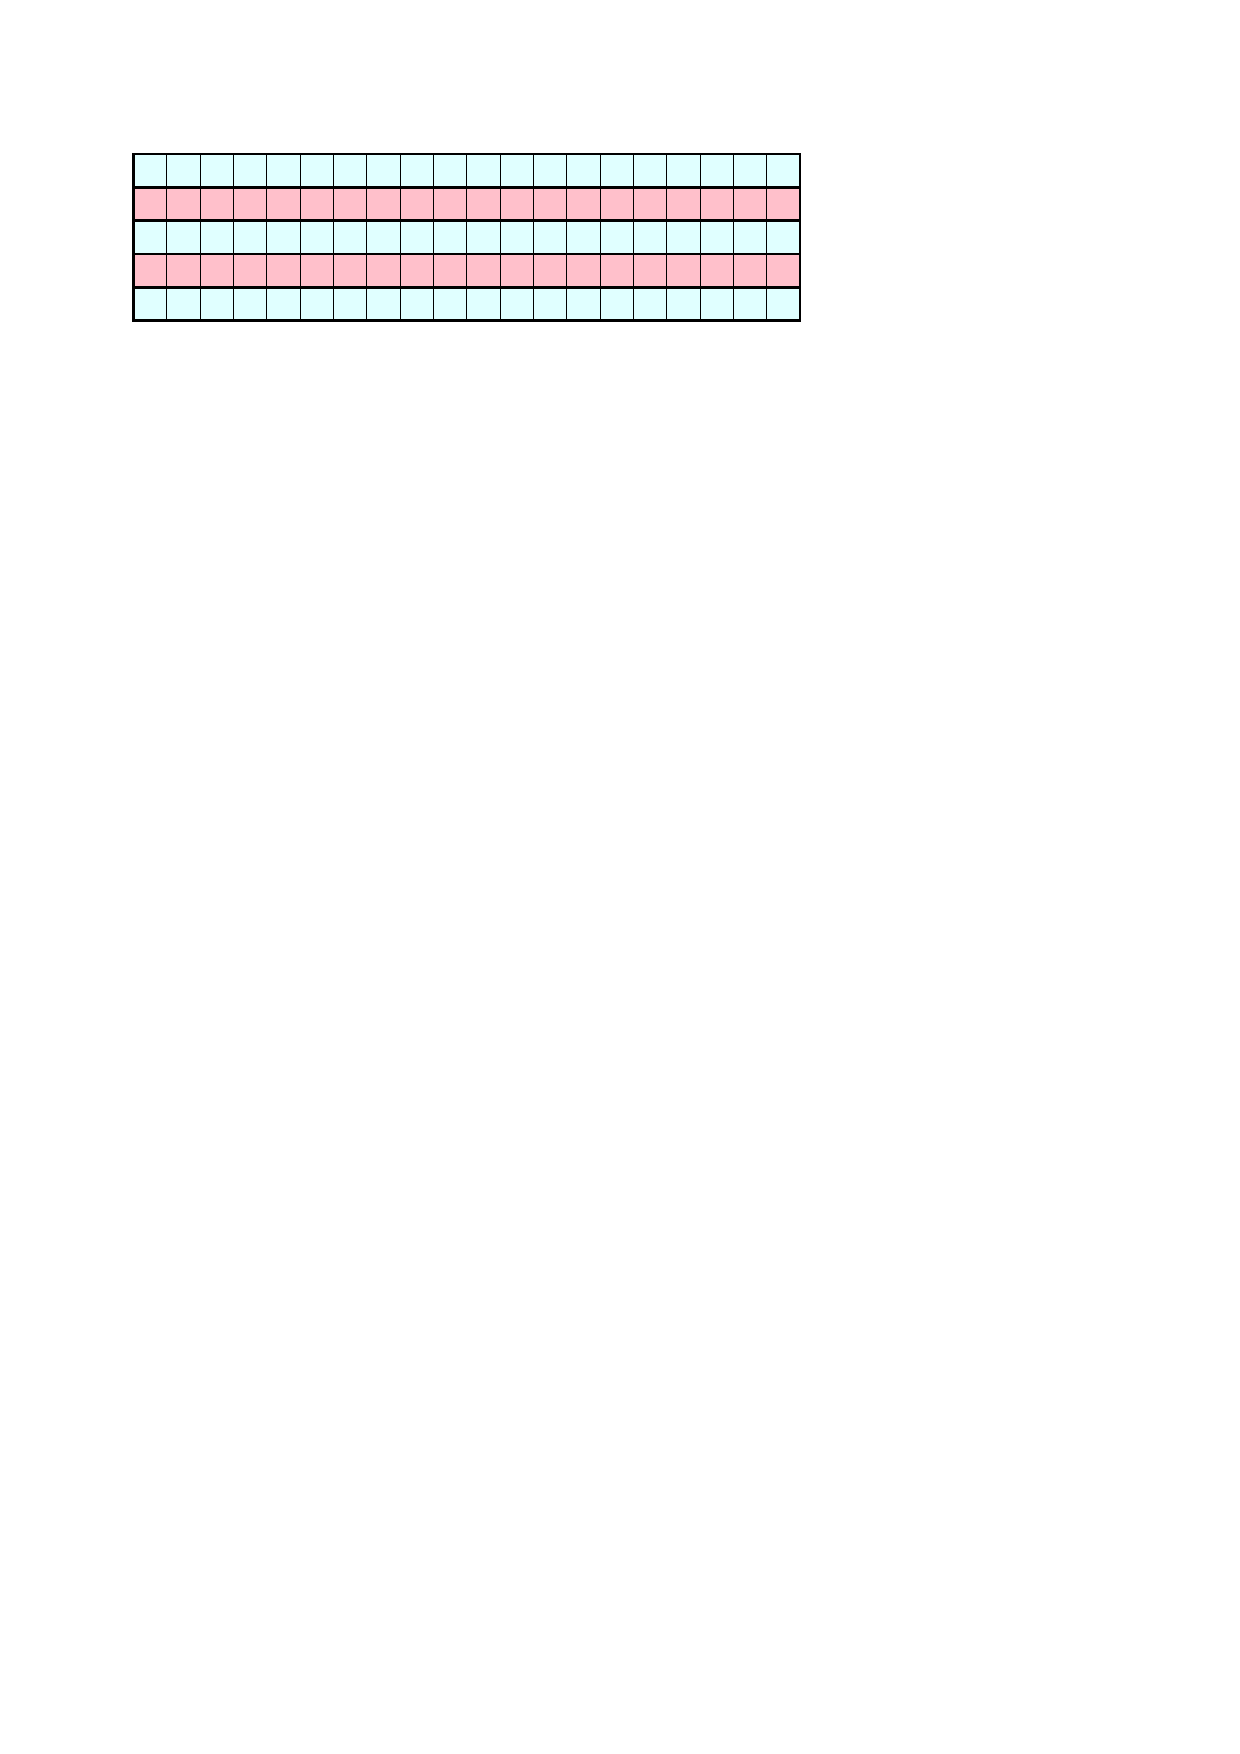
\includegraphics[width=18cm]{dimcoll-2}
\end{tabular}
\end{center}
%\vspace{0.2cm}
\end{minipage}
\hspace{1cm}
}
\end{textblock}

%%%%%%%%%%%%%%%%%%%%%%%%%%%%%%%%%%

\begin{textblock}{20}(11.8,5.5)
\Ovalbox{
\hspace{1cm}
\begin{minipage}{35.85cm}
\Head{Benchmarks}
\begin{center}
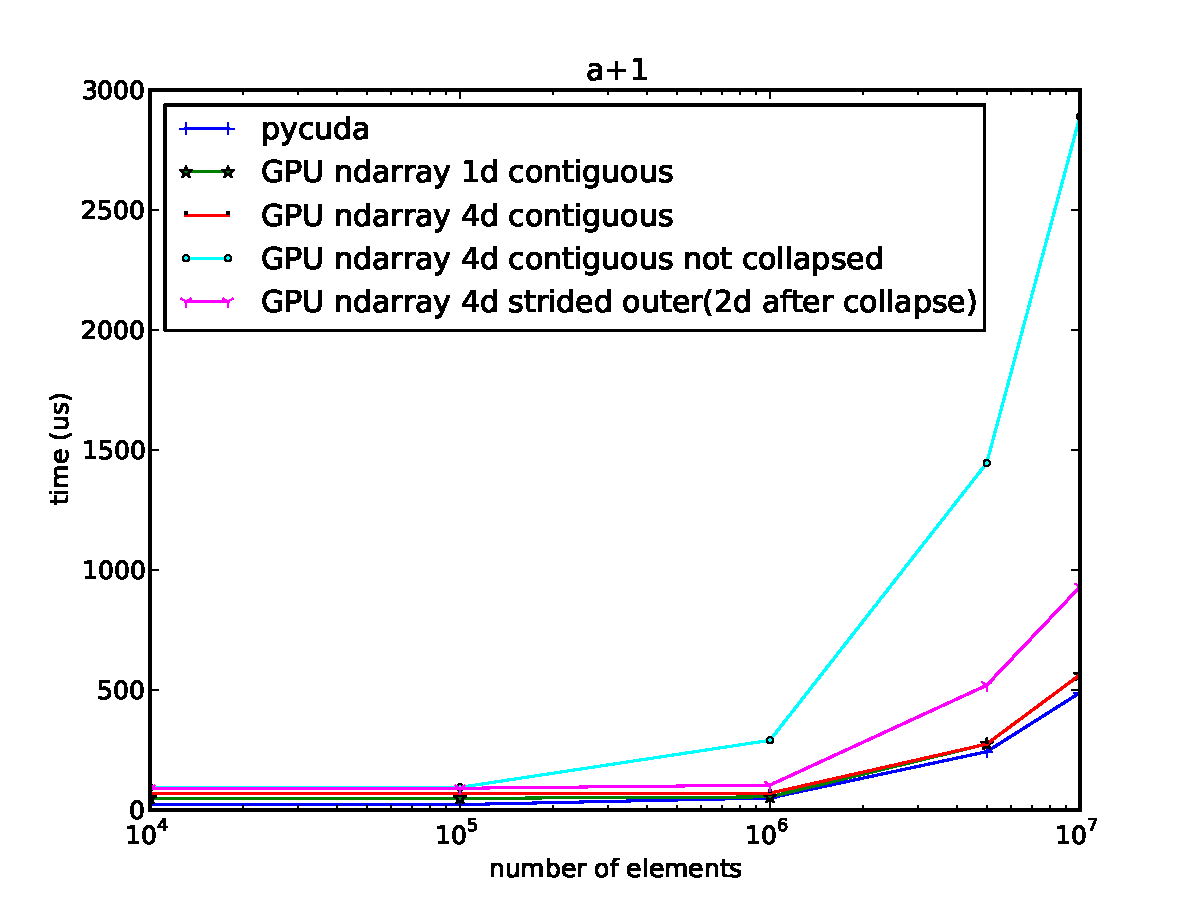
\includegraphics[width=0.49\textwidth]{ap1_no_alloc}
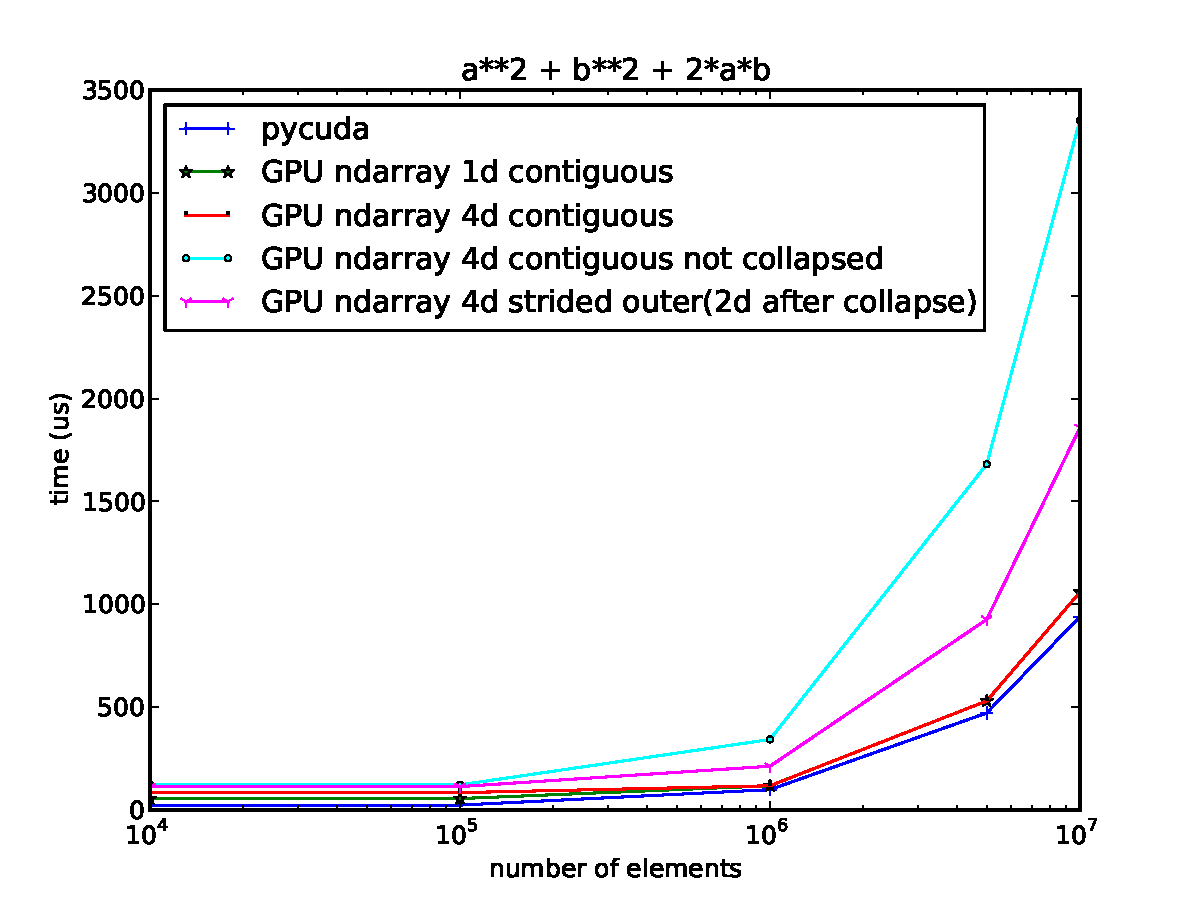
\includegraphics[width=0.49\textwidth]{a2pb2p2ab_no_alloc}
\end{center}
Speed for contiguous cases is similar to other implementations.
\vspace{0.8cm}
\end{minipage}
\hspace{1cm}
}
\end{textblock}

%%%%%%%%%%%%%%%%%%%%%%%%%%%%%%%%%%

\begin{textblock}{12}(11.8,7.6)
\Ovalbox{
\hspace{1cm}
\begin{minipage}{35.85cm}
\Head{Future Plans}
\begin{itemize}
\item Use in Theano/PyOpenCL/PyCUDA
\item Design and implement a good C/C++ interface
\item Find ways to lower the overhead
\item Use the implicit looping provided by CUDA and OpenCL
\item World domination!
\end{itemize}
\vspace{0.8cm}
\end{minipage}
\hspace{1cm}
}
\end{textblock}

%%%%%%%%%%%%%%%%%%%%%%%%%%%%%%%%%%

\begin{textblock}{6}(11.8,9.47)
\Ovalbox{
\hspace{1cm}
\begin{minipage}{35.85cm}
  \vspace{0.9cm}
\begin{thebibliography}{}
\bibitem[\protect\citename{Belkin and Niyogi}2003]{Belkin+Niyogi-2003}
Belkin, M. and Niyogi, P.\bibleft2003\bibright.
\newblock Laplacian eigenmaps for dimensionality reduction and data
  representation.
  \newblock {\em Neural Computation}, 15(6):1373--1396.

  \bibitem[\protect\citename{Ng, Jordan and Weiss}2002]{Ng2002}
Ng, A.~Y., Jordan, M.~I., and Weiss, Y.\bibleft2002\bibright.
\newblock On spectral clustering: Analysis and an algorithm.
\newblock In Dietterich, T.~G., Becker, S., and Ghahramani, Z., editors, {\em
  Advances in Neural Information Processing Systems 14}, Cambridge, MA. MIT
Press.

\bibitem[\protect\citename{Roweis and Saul}2000]{roweis00lle}
Roweis, S. and Saul, L.\bibleft2000\bibright.
\newblock Nonlinear dimensionality reduction by locally linear embedding.
\newblock {\em Science}, 290(5500):2323--2326.


\bibitem[\protect\citename{Tenenbaum, {de Silva} and
  Langford}2000]{Tenenbaum2000-isomap}
Tenenbaum, J., {de Silva}, V., and Langford, J.\bibleft2000\bibright.
\newblock A global geometric framework for nonlinear dimensionality reduction.
\newblock {\em Science}, 290(5500):2319--2323.

\bibitem[\protect\citename{Williams and Seeger}2000]{Williams+Seeger-2000}
Williams, C. and Seeger, M.\bibleft2000\bibright.
\newblock The effect of the input density distribution on kernel-based
  classifiers.
\newblock In {\em Proceedings of the Seventeenth International Conference on
  Machine Learning}. Morgan Kaufmann.
\end{thebibliography}{}
More references in the paper.

\vspace{0.82cm}
\end{minipage}
\hspace{1cm}
}
\end{textblock}


%\begin{textblock}{10}(0,0)
%\includegraphics{background.eps}
%\end{textblock}


%%%%%%%%%%%%%%%%%%%%%%%%%%%%%%%%%%%%%%%%%%%%%%%%%%%%%%%%%%%%%%%%%%%%%%%%%%%%%%%%%%%%%%%%%%%%%%%%%
%%% Minimization problem

%% \begin{textblock}{6}(14.5,6.7)
%% {\color{Green}
%% \Ovalbox{
%% {\color{Black}
%% \hspace{1cm}
%% \begin{minipage}{30cm}
%% \vspace{1cm}
%% \begin{center}
%% {\huge Minimization Problem}
%% \end{center}
%% \noindent
%% {\Large
%% Asymptotically, the spectral embedding for a kernel $K$ is the solution
%% of a sequential minimization problem, iteratively minimizing
%% the expected value of the loss criterion $L(x_i,x_j)$. More precisely,
%% with $\{(f_k,\lambda_k)\}_{k=1}^{q-1}$ already obtained,
%% one can recursively obtain $(f_q,\lambda_q)$  by minimizing
%%  \[
%%      \int (K(x_i,x_j)-\sum_{k=1}^q \lambda_k f_k(x)f_k(y))^2 p(x)p(y)dx dy
%%  \]
%% where by convention we scale $f_q$ such that $\int f_q(x)^2 p(x)=1$ (any other scaling
%% can be transferred into $\lambda_q$).
%% If the $K_n$ and the $f_{k,n}$ converge uniformly in probability, the Monte-Carlo
%% average of this criterion
%% \[
%%  \frac{1}{n^2}\sum_{i=1}^{n}\sum_{j=1}^n (K_n(x_i,x_j)-\sum_{k=1}^m \lambda_{k,n} f_{k,n}(x_i)f_{k,n}(x_j))^2
%% \]
%% converges in probability to the above asymptotic expectation.}
%% \vspace{1cm}
%% \end{minipage}
%% \hspace{1cm}
%% }}}
%% \end{textblock}
 
\end{document}


